\documentclass[12pt, a4paper]{article}
% \usepackage{background}
\usepackage[backend=bibtex,style=numeric,sorting=nyt]{biblatex}
\usepackage{fontspec}
\usepackage{graphicx}
\usepackage{hyperref}
\usepackage[figurename=Figure]{caption}
\counterwithin{figure}{section}
\usepackage[labelfont=bf]{caption}
\counterwithin{table}{section}
\usepackage{dirtree}
\usepackage{float} % needed for the H option for figures
\usepackage{subcaption}
\usepackage{amsfonts}
\usepackage{tikz} 
\usepackage[export]{adjustbox}
\usepackage{minted}
\usepackage{geometry}
\usepackage[framemethod=TikZ]{mdframed} 
\usepackage{enumitem}
\usepackage{makecell}
\usepackage{multirow}
\usepackage{tabularx}
\usepackage{csquotes}
\usepackage[croatian]{babel}
\usepackage{sectsty}
\usepackage{mdframed}
\usepackage{pdfpages}

\definecolor{LightGray}{gray}{0.9}

\hypersetup{
    colorlinks=true,
    linkcolor=blue,
    filecolor=magenta,      
    urlcolor=cyan,
    pdftitle={Peugeot Infotainment Project},
    }

\setmintedinline{frame=lines,
framesep=2mm,
baselinestretch=1.0,
fontsize=\footnotesize,
linenos}
\setminted{frame=lines,
framesep=2mm,
baselinestretch=1.0,
fontsize=\footnotesize,
bgcolor=LightGray,
linenos}
% page geom
\geometry{
    a4paper,
    left=25mm,
    right=20mm,
    top=25mm,
    bottom=25mm
}

\linespread{1.5}

% \setmainfont{Times New Roman}
% \setsansfont{Arial}
% \setmonofont{Courier New}


\addbibresource{sources.bib} % The filename of the bibliography

\begin{document}
\sectionfont{
  \fontsize{14}{16}
  \selectfont
}

\subsectionfont{
  \fontsize{14}{12}
  \selectfont
}

\subsubsectionfont{
  \fontsize{12}{9}
  \selectfont
}
\renewcommand\bibname{Literatura}
\renewcommand{\listingscaption}{Kod}
\newenvironment{code}{\captionsetup{type=listing}}{}
\selectlanguage{croatian}
\begin{titlepage}

\begin{center}
\fontsize{14}{16}
\selectfont
\textbf{SVEUČILIŠTE J.J. STROSSMAYER U OSIJEKU}

\bigskip
\vspace{9mm}
\fontsize{12}{12}
\selectfont
\textbf{FAKULTET ELEKTROTEHNIKE, RAČUNARSTVA I INFORMACIJSKH TEHNOLOGIJA OSIJEK}

\bigskip
\vspace{9mm}
\textbf{Sveučilišni studij}

\fontsize{11}{12}
\selectfont
\bigskip
\vspace{9mm}
\textbf{UGRADBENI RAČUNALNI SUSTAVI}

\bigskip
\vspace{9mm}
Profesor/mentor: \textbf{prof. dr. sc., Tomislav Keser}

\fontsize{12}{12}
\selectfont
\bigskip
\vspace{1cm}
\textbf{TEHNIČKA DOKUMENTACIJA PROJEKTA}

\fontsize{20}{16}
\selectfont
\bigskip
\vspace{9mm}
\begin{mdframed}[backgroundcolor=black!15]
  \begin{center}
    \textbf{PEUGEOT INFOTAINMENT SUSTAV}
  \end{center}
\end{mdframed}
\fontsize{11}{12}
\selectfont

\bigskip
\vspace{9mm}
Mislav Milinković, Ivan Brajinović

\bigskip
Akademska godina 2024/2025

\vspace*{\fill}
\textbf{Osijek, 19.09.2025.}
\end{center}
\end{titlepage}

\fontsize{12}{10}\selectfont
%=================================

\pagenumbering{gobble}

% Maksimalna dubina 2
\setcounter{tocdepth}{2}

\tableofcontents
\newpage

\newpage
\pagenumbering{arabic}

\section{Projekt}

\subsection{Uvod}

Cilj ovog projekta bio je izraditi pristupni modul za infotainment sustav
koji će se koristiti u vozilu Peugeot 206. Sam sustav sastoji se od dvaju glavnih dijelova:
pristupnog modula i računala. Pristupni modul izrađen je pločica vlastitog dizajna
temeljena na modulu ESP32 Wroom 32E. Pločica upravlja napajanjem,
komunikacijom s vozilom te komunikacijom s računalom.
Računalo čini Raspberry Pi 4 sa zaslonom osjetljivim na dodir
(DSI) i prilagođenom Linux distribucijom. Ono upravlja prikazom slike i zvuka.

\bigskip
\noindent
Ovaj projekt je proširenje postojećeg završnog rada `VAN protokol i njegova primjena u automobilima' \cite{mathos-rad}.

\begin{figure}[H]
  \begin{center}
    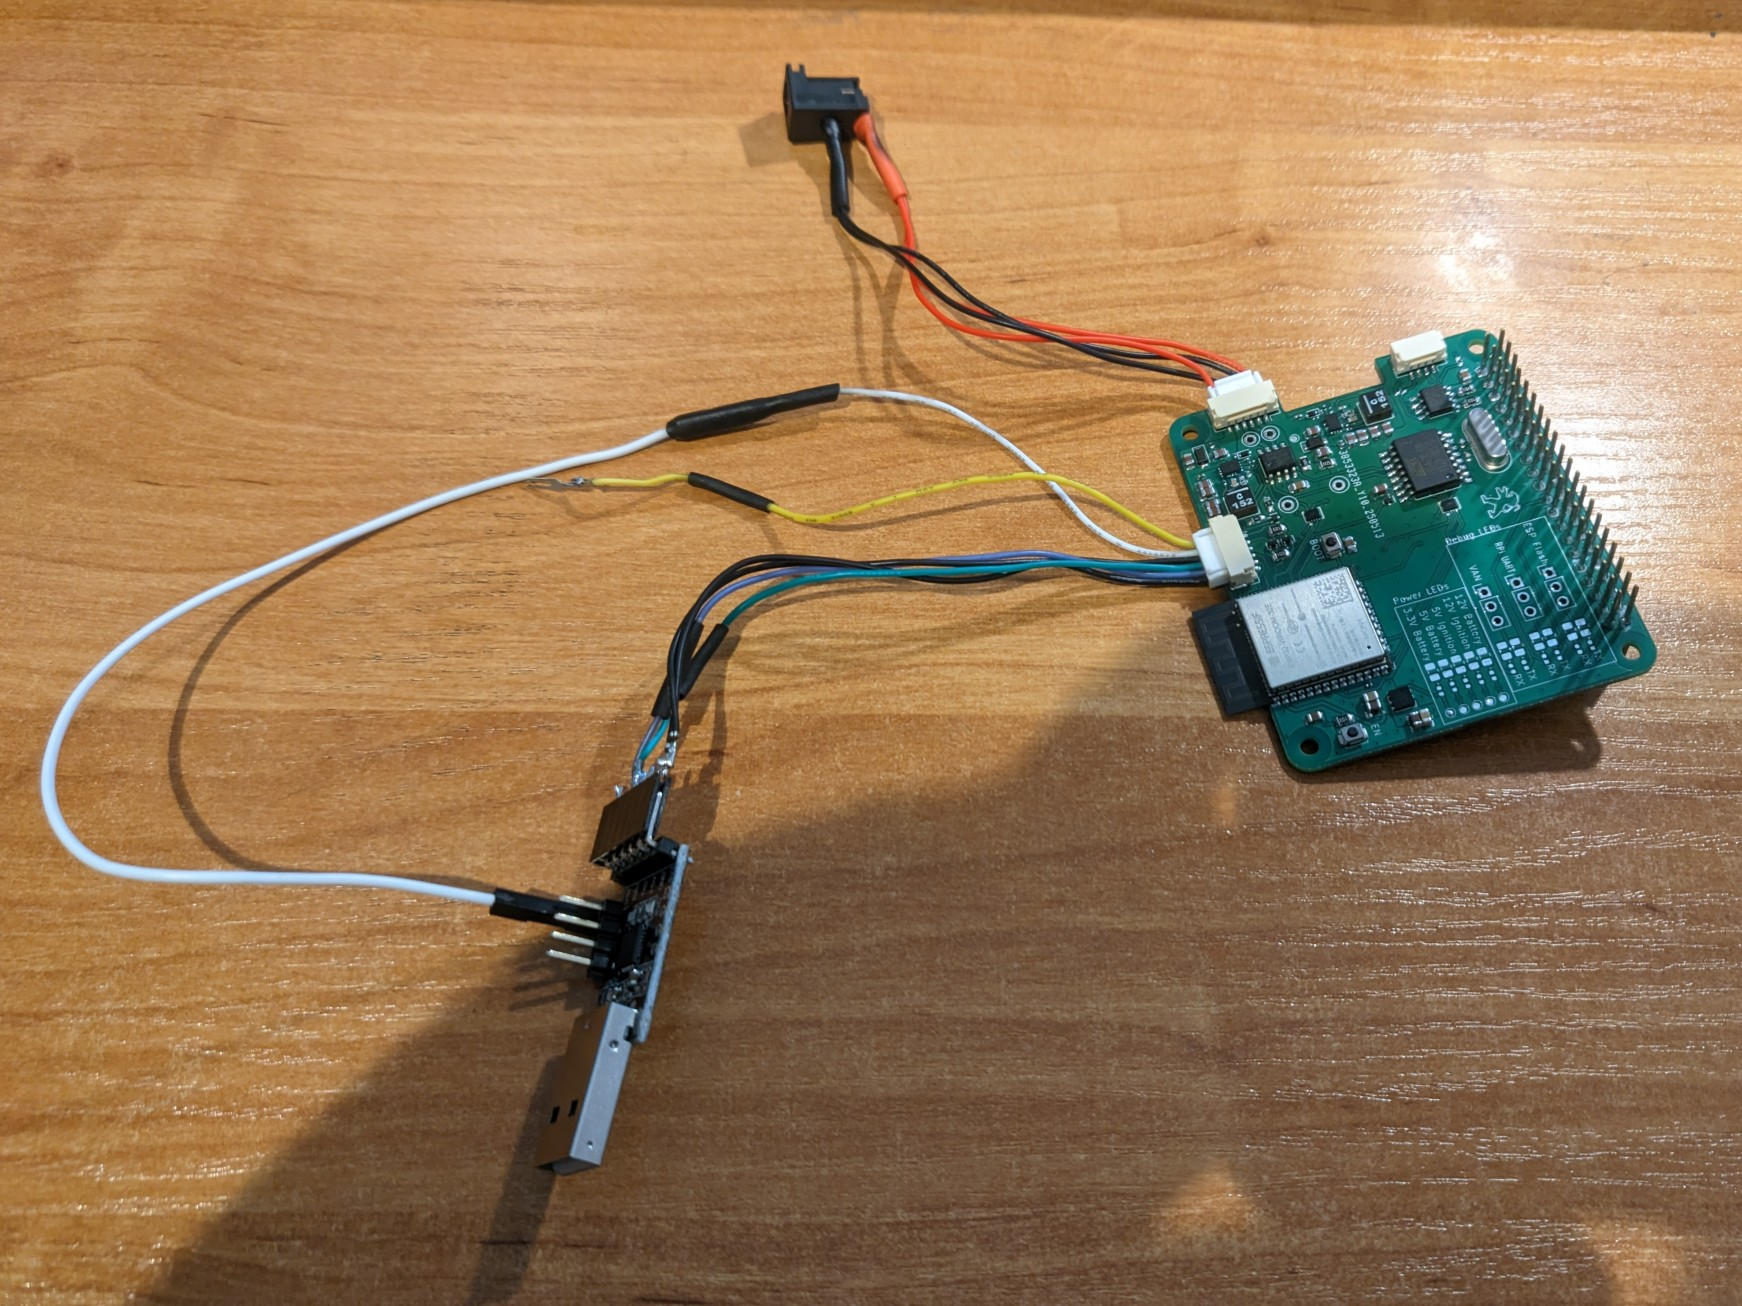
\includegraphics[width=0.75\textwidth]{images/PXL_20250530_205606724.jpg}
    \caption{Izgled pristupnog modula sa sklopovljem za programiranje.}
  \end{center}
\end{figure}

\subsection{Glavni izazovi}

Ovaj projekt ima dva, možda tri glavna izazova koje treba razmotriti. 
Najizraženiji je komunikacija s vozilom. Peugeot 206 ne koristi standardnu CAN sabirnicu, već nešto što se naziva VAN, vidi poglavlje \ref{sec:van_bus}. 
Taj komunikacijski standard danas je zastario, jer je korišten isključivo u vozilima Peugeot i Citroën tijekom ograničenog vremenskog razdoblja. 
Zbog toga gotovo da i ne postoji hardver koji može razumjeti taj protokol, 
a dokumentacije je približno jednako malo, pri čemu je većina napisana na francuskom jeziku. 
Stoga moramo izraditi vlastiti softver za primanje VAN okvira te pronaći način kako ih i slati.

\bigskip
\noindent
Drugi izazov odnosi se na napajanje. 
Imamo komponente koje zahtijevaju i 5 volti i 3,3 volta, kao i dva naponska voda: trajni izvor i uključivi izvor. 
Dodatni problem je \textbf{vrlo} šumovito i ponekad nestabilno ulazno napajanje, pa jeftini istosmjerni pretvarači (DC-DC) neće biti dovoljni.

\bigskip
\noindent
Posljednji izazov, a možda i najpodcijenjeniji, 
jest izrada pouzdane programske podrške (eng. \textit{firmwarea}) za sam pristupni modul. 
Modul ne treba samo analizirati VAN okvire, već mora upravljati vlastitim stanjem, pratiti stanje vozila, upravljati napajanjem i komunikacijom 
računala, kontrolirati režime mirovanja i upravljati vlastitim niskonaponskim stanjem, te, što je najvažnije, ne smije dolaziti do pada sustava.
\newpage
\section{Peugeot Infotainment sustav}\label{sec:van_bus}

\subsection{Principi i fizikalne zakonitosti}
VAN (eng. \textit{Vehicle Area Network}) je serijska komunikacijska sabirnica koju su razvili PSA grupa (Peugeot, Citroën) i Renault kao alternativu CAN sabirnici. 
Definirana je u ISO standardu \textbf{ISO 11519-3}. 
Koristi isti fizički sloj kao CAN sabirnica (diferencijalni par) i identičnu metodu arbitraže na sabirnici, 
ali se razlikuje u načinu pakiranja podataka.
Gotovo sve informacije navedene ovdje preuzete su iz Atmel TSS463C dokumentacije \cite{tss463c_datasheet}.

\bigskip
\noindent
Kao i CAN, VAN protokol koristi identifikatore za razlikovanje poruka i izvođenje arbitraže na sabirnici. 
Dodatno, omogućuje tzv. „odgovore unutar okvira” (eng. \textit{In-frame}), veće veličine poruka (28 bajtova umjesto 8 bajtova kao u CAN-u) 
te mogućnost izravne komunikacije s drugim uređajem.

\bigskip
\noindent
Podaci na VAN mreži pakiraju se u okvire. 
Okviri se sastoje od više dijelova: početka okvira (\textbf{SOF}), identifikatora poruke (\textbf{IDEN}), 
naredbe (\textbf{COM}), samih podataka (\textbf{DATA}), kontrolnog zbroja okvira (\textbf{FCS}), 
signala kraja podataka (\textbf{EOD}), signala potvrde (\textbf{ACK}) te signala kraja okvira (\textbf{EOF}).

\begin{table}[H]
    \centering
    \fontsize{10}{10}
    \selectfont
    \begin{tabular}{|c|c|c|c|c|c|c|c|c|c|c|}
        \hline
        \multirow{2}{*}{\makecell{SOF             \\ 10 TS}}  & \multirow{2}{*}{\makecell{IDEN \\ 12 bit \\ 15 TS}} & \multicolumn{4}{c|}{\makecell{Command \\ (4 bit, 5 TS)}} & \multirow{2}{*}{\makecell{DATA max. \\ 28 byte \\ 280 TS}} & \multirow{2}{*}{\makecell{FCS \\ 15 bit \\ 18 TS}} & \multirow{2}{*}{\makecell{EOD \\ 2 TS}} & \multirow{2}{*}{\makecell{ACK \\ 2 TS}} & \multirow{2}{*}{\makecell{EOF \\ 4 TS}} \\[7mm] \cline{3-6}
         &  & EXT & RAK & R/W & RTR &  &  &  &  & \\
        \hline
    \end{tabular}
    \caption{Oblik VAN okvira}
    \label{fig:van_frame_format}
\end{table}

\subsubsection{e-Manchester kodiranje}

Svi VAN okviri kodirani su pomoću unaprijeđenog Manchesterovog kodiranja (eng. \textit{Enhanced Manchester, e-Manchester}).
Kod e-Manchestera, nakon slanja tri NRZ bita, četvrti bit šalje se kao Manchesterov bit.
Slanje podataka na ovaj način omogućuje lakšu sinkronizaciju na sabirnici. 
Ovo je predvidljivija metoda ubacivanja bitova (eng. \textit{bit-stuffing}) u usporedbi s metodom korištenom na CAN sabirnici.

\bigskip
\noindent
U Tablici \ref{fig:van_frame_format} prikazan je broj bitova za svaki dio okvira, kao i broj vremenskih intervala (eng. \textit{Time Slots}, TS). 
Budući da Manchester bit zahtijeva dva vremenska intervala za prijenos, četiri bita u nizu kodirana e-Manchester metodom prenose se u 3 + 2 vremenska intervala.

\begin{figure}[H]
    \centering
    
\includegraphics[width=0.75\textwidth]{images/mux1-eman.pdf}
    \caption[]{e-Mancherster kodiranje \cite{mux1}}
    \label{fig:manchester_bits_mux1}
\end{figure}

\begin{figure}
    \centering
    
\includegraphics[width=0.5\textwidth]{images/manchester_bits.pdf}
    \caption{NRZ i Manchester bitovi. \cite{tss463c_datasheet}}
    \label{fig:manchester_bits_tss463_docs}
\end{figure}

\subsubsection{Poruke}

Uređaj ili modul povezan na mrežu može biti jednog od tri tipa:
\begin{itemize}
  \item Autonomni modul - glavni uređaj sabirnice. Može slati \textbf{SOF} niz, započeti prijenos podataka i primati poruke.
  \item Modul sa sinkronim pristupom - ne može slati \textbf{SOF} niz, ali može započeti prijenos podataka i primati poruke.
  \item Podređeni modul (eng. \textit{Slave}) - može slati poruke samo pomoću odgovora unutar okvira (eng. \textit{in-frame}) i također može primati poruke.
\end{itemize}

\begin{figure}
  \begin{center}
    
\includegraphics[width=0.75\textwidth]{images/ranking.pdf}
    \caption{Vrste modula, \cite{tss463c_datasheet}}
  \end{center}
\end{figure}

\noindent
VAN protokol podržava više tipova poruka. Razlikuju se pomoću polja identifikatora (\textbf{IDEN}) i naredbe (\textbf{COM}). Identifikator je dug 12 bita i slijedi ga 4 bita naredbe. Zbog načina na koji funkcionira arbitraža na sabirnici, manji identifikator ima prednost na sabirnici. Dok je vrijednost identifikatora potpuno proizvoljna, bitovi naredbe su strogo definirani i određuju tip poruke koja će se poslati na sabirnici:

\begin{itemize}
  \item EXT - uvijek 1
  \item RAK - `\emph{Request Acknowledge}' (zahtjev za potvrdom). Ako je 1, primatelj mora potvrditi primitak poruke. Ako je 0, signal ACK se ne šalje.
  \item R/W - `\emph{Read/Write}' (čitanje/pisanje). Označava smjer podataka. Ako je 0, radi se o poruci za pisanje (`\emph{write}'), gdje uređaj šalje podatke namijenjene drugom uređaju. Ako je 1, radi se o poruci za čitanje („\emph{read}”), što podrazumijeva zahtjev za podacima i očekuje odgovor.
  \item RTR - `\emph{Remote Transmission Request}' (zahtjev za daljinskim prijenosom). Ako je 0, poruka sadrži podatke. Ako je 1, poruka ne sadrži podatke i implicira zahtjev za odgovor unutar okvira (in-frame response). Kombinacija R/W = 0 i RTR = 1 je zabranjena na sabirnici.
\end{itemize}

\subsubsection{Vrste poruka}
\label{subsec:message-types}

Ovdje ćemo navesti tipove okvira relevantne za ovaj projekt. Postoje i drugi, ali koristimo samo ove.

\smallskip
\noindent
Podsjetnik: Dominantno = 0, Recesivno = 1.

\paragraph{Normalni okvir}

Najjednostavniji tip okvira. Jedan modul šalje cijeli okvir s podacima, te može, ali ne mora, zatražiti potvrdu (ACK). 
U slučaju da se potvrda ne traži, poruka se tretira kao poruka za emitiranje (eng. \textit{broadcast}).

\begin{figure}[H]
    \centering
    
\includegraphics[width=\textwidth]{images/normalframe_ack.pdf}
    \caption{Prijenos normalnog okvira sa ACK, \cite{tss463c_datasheet}}
    \label{fig:normal_frame_ack}
\end{figure}

\begin{figure}[H]
    \centering
    
\includegraphics[width=\textwidth]{images/normalframe_noack.pdf}
    \caption{Prijenos normalnog okvira bez ACK, \cite{tss463c_datasheet}}
    \label{fig:normal_frame_noack}
\end{figure}

\paragraph{Zahtjev sa trenutnim odgovorom}
\label{p:immediate-reply}

Ovo je jedini okvir u kojem podređeni modul (eng. \textit{slave}) može slati podatke. 
Jedina razlika na sabirnici je promjena stanja bita R/W u odnosu na normalni okvir.
Glavni modul sabirnice (eng. \textit{bus master}) generira \textbf{SOF}, inicijator generira identifikator i prva tri bita naredbe, te signal ACK. 
Ostalo (RTR, podaci i kontrolnu sumu) generira modul koji odgovara.

\begin{figure}[H]
\centering

\includegraphics[width=\textwidth]{images/immediate_reply.pdf}
\caption{Ilustracija prijenosa zahtjeva sa trenutnim odgovorom, \cite{tss463c_datasheet}}
\label{fig:immediate_reply_frame}
\end{figure}

\subsubsection{VAN mreža}

Više modula možemo povezati zajedno kako bismo stvorili mrežu. 
Također je moguće povezati više mreža i koristiti pristupni modul (eng. \textit{gateway}) za usmjeravanje podataka između mreža. 
U vozilu Peugeot 206 imamo jednu CAN mrežu \emph{CAN Engine} i tri VAN mreže: \emph{VAN Comfort}, \emph{VAN Body 1} i \emph{VAN Body 2}.

\noindent
Raspored mreža prikazan je na slici \ref{fig:van_can_network}. Tamo također možemo vidjeti pristupni modul, BSI. Ovaj modul prisutan je u svim vozilima PSA grupe. 
Konkretni BSI dolazi iz generacije AEE2001, jedine generacije koja koristi VAN sabirnicu. Druge generacije, AEE2004 i AEE2010, koriste isključivo CAN.
Naš infotainment sustav bit će spojen umjesto CD mjenjača, modul broj 8415 na slici \ref{fig:van_can_network} na \emph{VAN Comfort} sabirnici.

\begin{figure}[H]
  \begin{center}
    
\includegraphics[width=0.75\textwidth]{images/vannetwork.pdf}
    \caption{Pregled VAN i CAN mreže u Peugeot 206 automobilu \cite{sedre}}
    \label{fig:van_can_network}
  \end{center}
\end{figure}

Na slici \ref{fig:block_diagram_2_1} je prikazan block dijagram idejnog rješenja iz kojeg se mogu prepoznati tri dijela, kao i dio koji je centralni za ovaj projekt. Mikroupravljač je zadužen i za komunikaciju s računalom automobila, obradu dobivenih informacija te za njihov prikaz na ekranu.

\begin{figure}[H]
  \begin{center}
    
\includegraphics[width=0.75\textwidth]{images/block_diagram_2_1.pdf}
    \caption{Block dijagram idejnog rješenja}
    \label{fig:block_diagram_2_1}
  \end{center}
\end{figure}

\subsection{Pregled sklopovskog rješenja}

Na slici \ref{fig:block_diagram_2_2} se nalazi prikaz osnovnog sklopovskog dijagrama sustava. Glavni dio sustava je mikroupravljač koji ima ulogu komunikacije informacija s računalom automobila te obradu i prikaz tih istih informacija na ekranu. Kako mikroupravljač ne podržava VAN protokol, potrebno je koristiti upravljačke integrirane krugove koji pružaju sučelje s protokolom koji je podržan od strane mikroupravljača. Za slučaj da se ne pronađe upravljač koji ne podržava diferencijalni VAN protokol, bit će potrebno koristiti tzv. VAN Transciever kako bi preveli TTL logiku u diferencijalni par. Također zbog dodatne funkcionalnosti prikaza vremena na ekranu, potrebno je dodati RTC integrirani krug čija je zadaća praćenje stvarnog vremena te komunikacija istog s mikroupravljačem.

\begin{figure}[H]
  \begin{center}
    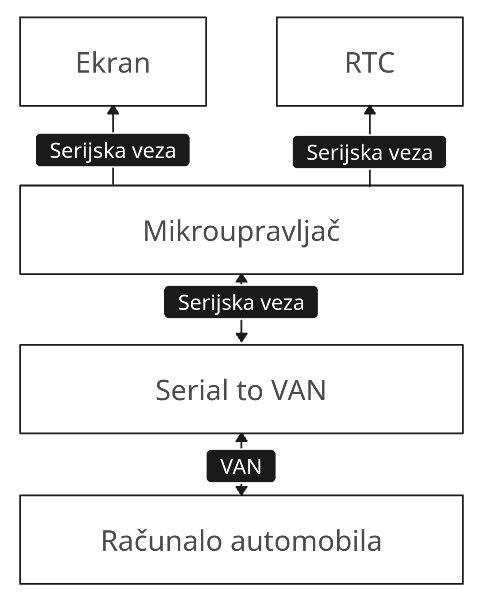
\includegraphics[width=0.75\textwidth]{images/block_diagram_2_2.png}
    \caption{Osnovni blok dijagram sklopovskog rješenja}
    \label{fig:block_diagram_2_2}
  \end{center}
\end{figure}

\subsection{Prijedlog programskog rješenja}
Na slici \ref{fig:block_diagram_2_3} je prikazan blok dijagram programskog rješenja koji daje abstraktan uvid u moguće programsko rješenje. Glavni program bi se vrtio na mikroupravljaču ESP32 koji je odgovaran za slanje i primanje paketa na VAN mreži tj. odgovaran je za komunikaciju s računalom automobila. Nadalje, pored toga je potrebno riješiti problem upravljanja potrošnjom energije i uvijetnog paljenja sustava tj. postavljanjem dijelova sustava u aktivno stanje ili stanje mirovanja. I na kraju je potrebno dobivene informacije obraditi te prikazati na ekranu.

\begin{figure}[H]
  \begin{center}
    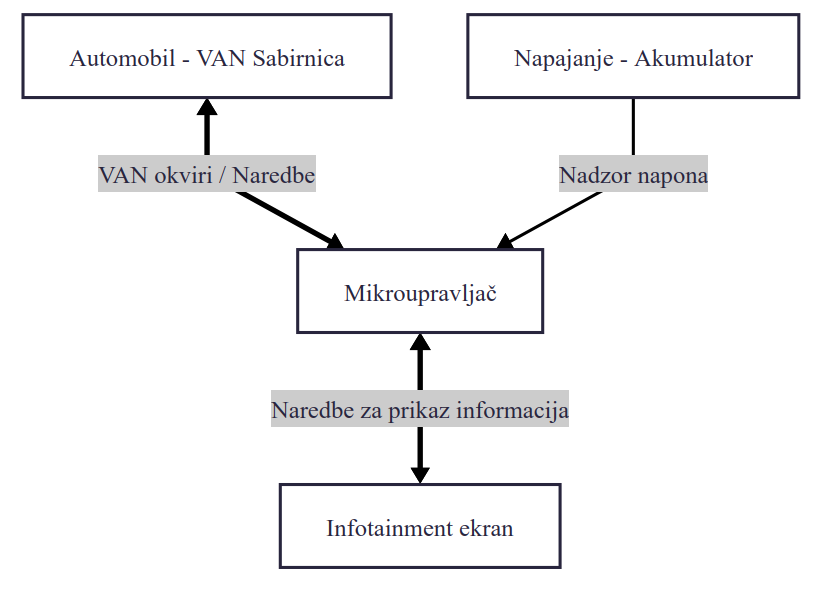
\includegraphics[width=0.75\textwidth]{images/block_diagram_2_3.png}
    \caption{Osnovni blok dijagram programskog rješenja}
    \label{fig:block_diagram_2_3}
  \end{center}
\end{figure}


\newpage

\section{Realizacija Peugeot Infotainment sustava}
\subsection{Korištene komponente, alati i programska podrška}
% ESP32
\paragraph{ESP32 - WROOM32E} glavni mikroupravljač sustava. Komunicira s računalom automobila, obrađuje zaprimljene informacije te ih prosljeđuje RPi mikroupravljaču.
% RPi
\paragraph{RPi 4} prihvaća i obrađuje dobivene informacije od ESP mikroupravljača te ih prikazuje na ekranu.
% RTC
\paragraph{RTC DS3231MZ} broji trenutno vrijeme koje se komunicira s RPi mikroupravljačem u svrhu prikaza istog na ekranu.
% TSS
\paragraph{TSS463C} integrirani strujni krug koji omogućuje jednostavno komuniciranje s VAN mrežom preko SPI sučelja. Apstrahira sam VAN protokol koji je kompleksan te ubrzava razvoj.
% MCP
\paragraph{MCP2551}je integrirani strujni krug koji pretvara naponske razine logičkih razina VAN sabirnice u diferencijalni signal.
% Level shifteri
\paragraph{NTS0104}je integrirani strujni krug koji prevodi naponske razine signala.
% 5V voltage reg
\paragraph{MP8759GD1}je integrirani strujni krug koji služi kao regulator napona. U ovom konkretnom slučaju se koristi za pretvorbu napona od 12 V u 5 V.
% 3v3 voltage reg
\paragraph{NCP691} je integrirani strujni krug koji služi kao regulator napona za 3.3 V.
\paragraph{ESP-IDF programski paket} razvijen od Espressif-a se koristi za programiranje za ESP mikroupravljača.

\subsection{Realizacija konstrukcijskog i sklopovskog rješenja}

% detaljna elektronična shema te detaljno objašnjenje iste

% ESP
Napaja se s 3.3 V sa stalnog izvora napajanja (\ref{fig:3v3_reg}), EN nožica je spojena preko otpornika na napon napajanja (eng. \textit{pull-up}) kako bi se omogućio rad mikroupravljača. Shema mikroupravljača je prikazana na slici \ref{fig:esp32}.
\begin{figure}[H]
    \centering
    
\includegraphics[width=0.65\textwidth]{images/sch_esp32.pdf}
    \caption[]{Pregled sheme - ESP32 mikroupravljač}
    \label{fig:esp32}
\end{figure}

% dugmad za programiranje
Prije samog procesa prijenosa koda na ESP, isti se mora postaviti u određeni način rada gdje je spreman prihvatiti programski kod. Zbog toga se koristi gumb SW2A koji kad je pritisnut dovodi nisku naponsku razinu na GPIO0 što je uvijet kod ponovnog pokretanja mikroupravljača za odlazak u spomenuti način rada. Zbog lakšeg ponovnog pokretanja, implementiran je još jedan gumb za ponovno pokretanje koji, kad se pritisne, dovede nisku naponsku razinu na EN nožicu. Shema gumbova se nalazi na slici \ref{fig:programming_buttons}.
\begin{figure}[H]
    \centering
    
\includegraphics[width=0.9\textwidth]{images/sch_prog_buttons.pdf}
    \caption[]{Pregled sheme - Gumbovi za programiranje}
    \label{fig:programming_buttons}
\end{figure}

% tranzistori za programiranje
Dugmad na slici \ref{fig:programming_buttons} se koriste za ručno tj. fizičko programiranje. Međutim, kako bi omogućili programsko programiranje tj. omogućili programiranje mikroupravljača bez fizičkog pritiskanja gumba, implementirana su dva tranzistora koji pružaju programsko upravljanje naponskih razina nožica mikroupravljača. Shema tih tranzistora je prikazana na slici \ref{fig:programming_transistors}.
\begin{figure}[H]
    \centering
    
\includegraphics[width=0.55\textwidth]{images/sch_prog_npn.pdf}
    \caption[]{Pregled sheme - Tranzistori za programiranje}
    \label{fig:programming_transistors}
\end{figure}

% spojnica za programiranje
U svrhe programiranja je kreirano posebno sučelje koje koristi tranzistore za programiranje koji su prethodno spomenuti kako bi odabrali način rada mikroupravljača kao i UART serijski protokol za sam prijenos programskog koda. Shema sučelja je prikazana na slici \ref{fig:programming_header}.
\begin{figure}[H]
    \centering
    
\includegraphics[width=0.75\textwidth]{images/sch_prog_header.pdf}
    \caption[]{Pregled sheme - spojnica za programiranje}
    \label{fig:programming_header}
\end{figure}


% pretvarač naponskih razina opće namjene
Kako imamo komponente koje rade na različitim naponskim razinama, potrebno je upotrijebiti pretvarač naponskih razina kako bi se pouzdano i bez razmišljanja o pregaranju, razmjenjivale informacije između njih. Pretvarač naponskih razina na slici \ref{fig:level_shifter_A} vrši pretvorbu na signalima prekida TSS integriranog kruga te na liniji dolaznih podataka VAN sabirnice.
\begin{figure}[H]
    \centering
    
\includegraphics[width=0.9\textwidth]{images/sch_gp_level_shifter.pdf}
    \caption[]{Pregled sheme - pretvarač naponskih razina A}
    \label{fig:level_shifter_A}
\end{figure}

% sučelje za spajanje na mrežu automobila
TSS463C je VAN upravljački integrirani krug koji se koristi za komunikaciju sa sustavom automobila. Komunicira s ESP mikroupravljačem putem SPI serijskog protokola. Od periferije sadržava 8 MHz oscilator koji je neophodan za rad integriranog kruga. Sa sustavom automobila kominicira preko VAN protokola (nožice 11 i 12). Shema spoja je prikazana na slici \ref{fig:tss}. 
\begin{figure}[H]
    \centering
    
\includegraphics[width=0.75\textwidth]{images/sch_tss.pdf}
    \caption[]{Pregled sheme - TSS}
    \label{fig:tss}
\end{figure}

% TSS oscilator
Slika \ref{fig:tss_osci} pokazuje oscilator koji je spojen na TSS463C integrirani krug.
\begin{figure}[H]
    \centering
    
\includegraphics[width=0.55\textwidth]{images/sch_tss_osci.pdf}
    \caption[]{Pregled sheme - TSS oscilator}
    \label{fig:tss_osci}
\end{figure}

% TSS level shifter
Kako TSS ne može direktno komunicirati s mikroupravljačem, između njih je postavljen pretvarač naponskih razina kako bi preveo 5 V signale od TSS-a u 3.3 V signale koje ESP očekuje. Shema spoja je prikazana na slici \ref{fig:level_shifter_B}.
\begin{figure}[H]
    \centering
    
\includegraphics[width=0.85\textwidth]{images/sch_tss_level_shifter.pdf}
    \caption[]{Pregled sheme - Pretvarač naponskih razina B}
    \label{fig:level_shifter_B}
\end{figure}

% TSS Reset transistor
Kao mehanizam za ponovno pokretanje TSS integriranog kruga preko ESP mikroupravljača, ugrađen je N kanalni unipolarni tranzistor koji je spojen na nožicu za ponovno pokretanje TSS integriranog kruga. Kako je ta nožica aktivna na nisku naponsku razinu, kad je tranzistor u zasićenju, nožica se spaja na uzemljenje te se tako TSS integrirani krug ponovno pokreće.
\begin{figure}[H]
    \centering
    
\includegraphics[width=0.6\textwidth]{images/sch_tss_reset.pdf}
    \caption[]{Pregled sheme - Tranzistor za ponovno pokretanje TSS-a}
    \label{fig:tss_reset}
\end{figure}

% MCP
Integrirani krug koji prevodi TTL signale u diferencijalni par.
\begin{figure}[H]
    \centering
    
\includegraphics[width=0.9\textwidth]{images/sch_mcp.pdf}
    \caption[]{Pregled sheme - MCP}
    \label{fig:mcp}
\end{figure}

% MCP reset transistor 
Kao mehanizam ponovnog pokretanja MCP integriranog kruga preko ESP mikroupravljača, implementiran je n kanalni unipolarni tranzistor koji je spojen na nožicu za ponovno pokretanje MCP integriranog kruga. Kako je ta nožica aktivna na nisku naponsku razinu, kad je tranzistor u stanju zasićenja, nožica se spaja na pull-down otpornik te se tako MCP integrirani krug ponovno pokreće.
\begin{figure}[H]
    \centering
    
\includegraphics[width=0.65\textwidth]{images/sch_mcp_reset.pdf}
    \caption[]{Pregled sheme - Tranzistor za ponovno pokretanje integriranog kruga MCP...}
    \label{fig:mcp_reset}
\end{figure}

% Regulator napona stalnog izvora - direktan spoj na bateriju | potencijalno spojiti s drugim regulatorom 12 V -> 5 V
Strujni krug je preuzet iz tehničkog lista \cite{MP8759GD1_datasheet} integriranog kruga MP8759GD1, na slici 11.Na strujnom krugu se nalazi jedna TVS dioda kako bi osigurala ulaznu nožicu od previsokog napona kao i razne vrijednosti kondenzatora čija je uloga filtriranje i peglanje oblika ulaznog napona.
Na izlazu se nalaze isto tako kondenzatori za filtriranje i peglanje oblika izlaznog napona. 
Kako je riječ o regulatoru napona koji nije ograničen na jednu vrijednost izlaznog napona, potrebno je odabrati željeni izlazni napon. A to je nešto što se radi na nožici 7 običnog naponskog djelila R111 i R109. Tablica s parovima vrijednosti za željene vrijednosti izlaznog napona se nalaze u tehničkom listu \cite{MP8759GD1_datasheet} na stranici 16.
\begin{figure}[H]
    \centering
    
\includegraphics[width=1\textwidth]{images/sch_5v_reg.pdf}
    \caption[]{Pregled sheme - Regulator napona stalnih 5 V}
    \label{fig:constant_5v_regulator}
\end{figure}

% 3v3 regulator napona
Linearni regulator napona koji kao ulaz prima 5 V i na izlazu daje 3.3 V. Posjeduje par kondenzatora na ulazu i izlazu u svrhu filtriranja i peglanja napona.
\begin{figure}[H]
    \centering
    
\includegraphics[width=0.9\textwidth]{images/sch_3v3_reg.pdf}
    \caption[]{Pregled sheme - 3.3 V regulator napona}
    \label{fig:3v3_reg}
\end{figure}


% ADC za mjerenje razine napona baterije automobila
Kako bi se mjerila razina napona baterije automobila, korišten je obični djeljitelj napona realiziran pomoću dva otpornika. Kako bi se što više ograničila struja koja ovim djeliteljem teče odabrane su vrijenosti otpornika u rasponu od stotina tisuća ohm-a. Omjer otpora koji je korišten je 4:1 tj. na nožici ESP-a će biti 1/5 napona baterije automobila.
\begin{figure}[H]
    \centering
    
\includegraphics[width=0.4\textwidth]{images/sch_battery_adc.pdf}
    \caption[]{Pregled sheme - Djeljitelj napona baterije}
    \label{fig:car_battery_voltage_divider}
\end{figure}

% sve LED za otklanjanje žohara
% Žohari, kao neminovna pojava se ne mogu izbjeći ali se može olakšati njihov pronalzak. Iz tog razloga se koriste LE diode kao bi pomoću njih brzo i jednostavno se otkrila njihova pojava.
LE diode za detekciju grešaka su postavljene na mnogim bitnim mjestima kako bi uprzale postupak razvoja. Svaka LED posjeduje otpornik koji ograničava struju koja prolazi kroz LED na 1 mA te se na njemu dešava preostali pad napona. \\
\begin{figure}[H]
    \centering
    
\includegraphics[width=0.55\textwidth]{images/sch_power_debug_led.pdf}
    \caption[]{Pregled sheme - LE diode za detekciju i otklanjanje žohara}
    \label{fig:debug_leds_power}
\end{figure}
\begin{figure}[H]
    \centering
    
\includegraphics[width=0.7\textwidth]{images/sch_UART_debug_led.pdf}
    \caption[]{Pregled sheme - LE diode za detekciju i otklanjanje žohara na UART sabirnici}
    \label{fig:debug_leds_uart}
\end{figure}
\begin{figure}[H]
    \centering
    
\includegraphics[width=0.4\textwidth]{images/sch_van_debug_led.pdf}
    \caption[]{Pregled sheme - LE diode za detekciju i otklanjanje žohara na VAN sabirnici}
    \label{fig:debug_leds_van}
\end{figure}
% RPi UART debug
\begin{figure}[H]
    \centering
    
\includegraphics[width=0.4\textwidth]{images/sch_rpi_uart.pdf}
    \caption[]{Pregled sheme - Shema spoja LE dioda za detekciju i otklanjanje žohara na UART sabirnici koja povezuje RPi i ESP32}
    \label{fig:rpi}
\end{figure}
% RPi header
Spojnica s 40 nožica karakteristična za RPi liniju mikroupravljača je prikazana na slici \ref{fig:rpi_header}. Preko ove spojnice se UART sabirnicom povezuju ESP i RPi. I2C sabirnica se koristi za komunikaciju RPi mikroupravljača s RTC modulom te LCD ekranom. Kao opcija su ucrtane ali ne postavljene komponente otpornika R13 i R14.
\begin{figure}[H]
    \centering
    
\includegraphics[width=0.7\textwidth]{images/sch_rpi_header.pdf}
    \caption[]{Pregled sheme - Spojnica za RPi mikroupravljač}
    \label{fig:rpi_header}
\end{figure}

% RPi RTC
Integrirani krug DS3231MZ obnaša ulogu RTC-a. Spoj je odrađen prema naputcima iz tehničkog lista \cite{rtc_datasheet}. Nožice 1 i 3 se spajaju preko otpornika na napon napajanja kako se ne koriste, nožice 7 i 8 su spojene na I2C sabirnicu RPi mikroupravljača. Postoji stalan izvor napajanja te drugi koji je aktivan kad se auto probudi.
\begin{figure}[H]
    \centering
    
\includegraphics[width=0.75\textwidth]{images/sch_rpi_rtc.pdf}
    \caption[]{Pregled sheme - Shema spoja RTC modula za RPi mikroupravljač}
    \label{fig:rpi_rtc}
\end{figure}


% spojnica za LCD display
Na slici \ref{fig:lcd_power} je prikazana JST spojnica za LCD ekran kojeg upogoni RPi. Nudi pristupne točke na I2C sabirnicu kao i izvor napajanja od 5 V.
\begin{figure}[H]
    \centering
    
\includegraphics[width=0.75\textwidth]{images/sch_lcd_pwr.pdf}
    \caption[]{Pregled sheme - Spojnica za LCD ekran}
    \label{fig:lcd_power}
\end{figure}
% kabal za spajanje na VAN mrežu JST -> Mini Iso Blue
 

% mini iso blue - van komunikacija
Na slici \ref{fig:mini_iso_blue} je JST spojnica koja omogućava spajanje na VAN mrežu automobila. 
\begin{figure}[H]
    \centering
    
\includegraphics[width=0.75\textwidth]{images/sch_jst_van.pdf}
    \caption[]{Pregled sheme - Spojnica za VAN mrežu automobila}
    \label{fig:mini_iso_blue}
\end{figure}

Na slikama \ref{fig:pcb_front} i \ref{fig:pcb_back} se nalazi izgled printane tiskane pločice koja predstavlja sklopovski dio projekta. Sve komponente se nalaze sa iste strane kako bi se olakšao i ubrzao proces lemljenja. Radi lakšeg snalaženja je svaka značajnija komponenta naznačena na slici. Oznake se manifestiraju bojama kao i pratećim tekstom. Spojnica J3 označava mjesto gdje se spaja LCD ekran, J2 označava mjesto povezivanja projekta sa mrežom auta te J7 označava mjesto sa kojeg je moguće programiranti ESP32 mikroupravljač.

\begin{figure}[H]
    \centering
    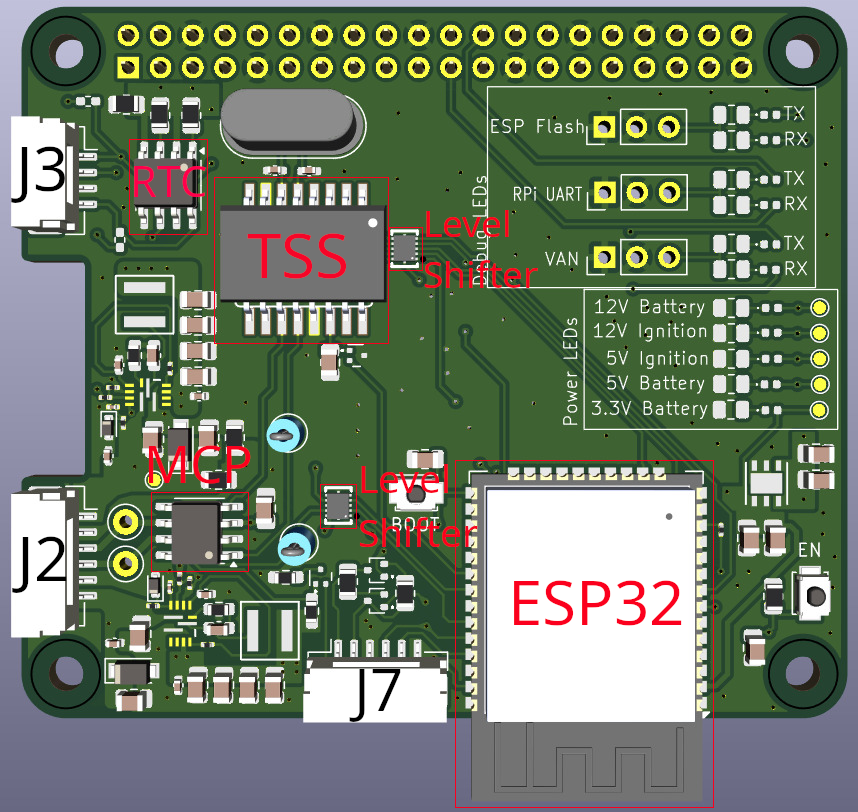
\includegraphics[width=0.75\textwidth]{images/pcb_front.png}
    \caption[]{Izgled prototipa - PCB prednja strana}
    \label{fig:pcb_front}
\end{figure}
\begin{figure}[H]
    \centering
    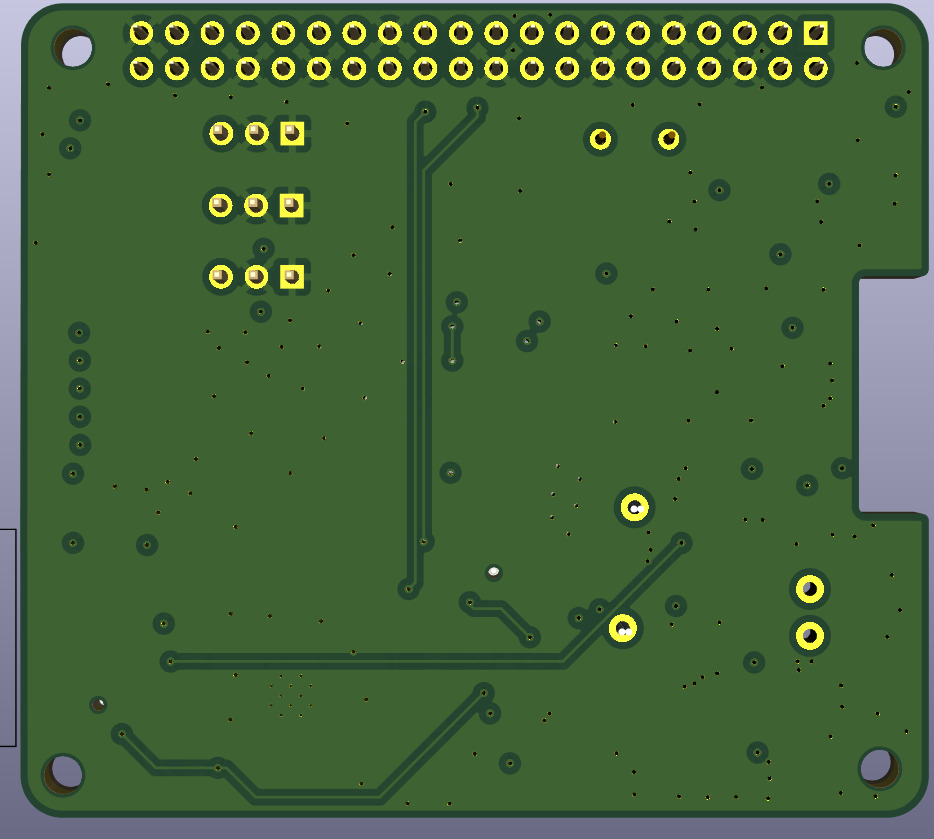
\includegraphics[width=0.75\textwidth]{images/pcb_back.jpeg}
    \caption[]{Izgled prototipa - PCB zadnja strana}
    \label{fig:pcb_back}
\end{figure}


\bigskip
\noindent
% Nožice 13 do 17, koji služe za podatke i napajanje, povezani su s pristupnim modulom pomoću JST GH spojnice s 6 nožica, dok su nožice 18 do 20 spojeni na 3.5 mm zvučni kabel i povezani s Raspberry Pi-jem. Budući da konvencija imenovanja razlikuje na Slikama \ref{fig:iso_conn_pinout} i \ref{fig:jst_van_pinout}, pogledajte tablicu \ref{tbl:iso-jst-legend} za spajanje.

\subsection{Realizacija programskog rješenja}

\begin{figure}[H]
    \centering
    
\includegraphics[width=1\textwidth]{images/block_diagram_3_3.png}
    \caption{Blok dijagram programskog rješenja}
    \label{fig:block_diagram_3_3}
\end{figure}

Pristupni modul je najvažniji dio ovog projekta jer se sučeljava s vozilom i odgovoran je za upravljanje napajanjem cijelog sustava. 
Modul prima i analizira VAN okvire, organizira podatke i zatim ih prosljeđuje infotainment računalu. 
Također obavlja i obrnuti proces: može primati podatke s infotainment računala i prenijeti odgovarajući VAN okvir na sabirnicu. 
upravljanje napajanjem također je važan dio programske podrške, budući da prekomjerna potrošnja u stanju mirovanja brzo iscrpljuje akumulator vozila. Detaljan blok dijagram je prikazan na slici \ref{fig:block_diagram_3_3} čije objašnjenje se nalazi u nastavku.

\subsubsection{Okvir i pristup}

Kao program za razvoj koristimo ESP-IDF programski okvir koji pruža Espressif. 
Okvir se temelji na operativnom sustavu FreeRTOS. Zbog prirode OS-a i programskog okruženja, programska podrška modula napisana je 
koristeći pristup temeljen na događajima.

\bigskip
\noindent
Koristimo sljedeće događaje kao osnovu za glavne petlje/zadatake:
\begin{itemize}
\item Primanje VAN okvira
\item Primanje UART podataka s računala
\item Promjena stanja vozila
\item Timer događaji
\item Glavni zadatak
\end{itemize}

\noindent
Budući da ESP32 ima dvije jezgre, jedna je posvećena isključivo primanju i analiziranju VAN okvira, jer su oni vrlo česti i ne želimo propustiti niti jedan.

\subsubsection{Primanje VAN okvira}

Za primanje VAN okvira potrebno je ručno čitati i vremenski pratiti stanja RX pina. 
Srećom, ESP32 ima sklopovski periferni uređaj koji upravo to omogućuje: RMT periferni uređaj. 
On može pratiti stanja GPIO pinova i mjeriti koliko dugo su u tom stanju. 
Nakon što postavimo pragove za minimalnu i maksimalnu duljinu signala, periferni uređaj može generirati prekid (eng. \textit{interrupt}) 
svaki put kada detektira sekvencu \textbf{EOF}.

\noindent
Kada se detektira sekvenca \textbf{EOF}, RMT periferijalni upravljački program generira prekid (eng. \textit{interrupt}). 
U okviru tog prekida, u red zadataka (eng. \textit{task queue}) modula za primanje VAN okvira postavljamo novi događaj i ponovno pokrećemo RMT. 
Modul za primanje VAN okvira preuzima primljene RMT podatke iz reda i analizira ih. 

VAN okvir rekonstruiramo bit po bit iz tog polja, uzimajući u obzir Manchester bitove. 
Nakon provjere kontrolnog zbroja (eng. \textit{checksum}), izdvajamo identifikator i podatke, 
stavljamo ih u novi međuspremnik i postavljamo u red glavnog zadatka (eng. \textit{Main task}) za daljnju obradu. 
Logika primanja inspirirana je Peter Pinterovom Arduino bibliotekom \cite{esp32_rmt_van} i prilagođena je arhitekturi naše programske podrške.

\subsubsection{Analiza VAN okvira}

Kada modul za primanje VAN okvira postavi novi događaj, glavni zadatak (eng. \textit{Main task}) 
poziva parser paketa koji provjerava identifikator i, ako je prepoznat, analizira podatke u globalne međuspremnike 
te postavlja odgovarajuće događaje u red glavnog zadatka ovisno o paketu koji se obrađuje. 
Velika većina poznatih dekodiranih VAN okvira dostupna je na web stranici Petera Pintera \cite{vanbus_packets}.

\subsubsection{Slanje VAN okvira}

Za slanje VAN okvira prema vozilu koristimo TSS463C. 
TSS je zapravo dodatnih 128 bajtova RAM-a kojima moramo upravljati, budući da moramo kontrolirati svu memoriju korištenu za slanje i primanje podataka.
Trenutno se TSS koristi samo za slanje paketa CD izmjenjivača kako bismo ga mogli emulirati, te za slanje zahtjeva za resetiranje stanja putnog računala. 
Poruke CD mijenjača su poruke s neposrednim odgovorom (vidi \ref{subsec:message-types}), dok je zahtjev za resetiranje stanja putnog računala normalni okvir s zahtjevom za potvrdom (ACK). 
Paketi CD mijenjača šalju se periodično, svake sekunde, inače će ugrađeni radio smatrati da CD mijenjač nije prisutan i onemogućiti ga.

\noindent
TSS komunicira preko SPI sučelja i malo je nezgrapan za korištenje, pa je napisan vlastiti upravljački program radi lakšeg rukovanja. 
Osim toga, postoji zaseban zadatak koji nadzire stanje TSS poruka i stavlja ih u red za slanje.

\subsubsection{UART komunikacija}

Informacijsko-zabavno računalo komunicira s ESP32 preko UART sučelja. Razlog korištenja UART-a je njegova jednostavnost. 
ESP32 uglavnom šalje podatke računalu, ali također može primati zahtjeve s računala.

\noindent
UART kod se izvodi u vlastitom zadatku koji prima događaje iz drugih zadataka i također može slati događaje glavnom zadatku. 
Kada glavna petlja (eng. \textit{Main loop}) detektira promjenu u globalnim međuspremnicima podataka (primljen VAN okvir, promjena napona akumulatora, itd.), 
postavlja odgovarajući događaj u UART zadatak s podacima koji se šalju računalu. 
Protokol i strukture podataka su inspirirane MSP protokolom korištenim u programskoj podršci upravljača leta na FPV dronovima.

\subsubsection{Upravljanje događajima i zadacima}

Programska podrška koristi nekoliko zadataka koji se izvode u vlastitim petljama i čekaju događaje iz više redova. Ukupno postoje 4 globalna reda u programskoj podršci, po jedan za svaku glavnu komponentu:
\begin{itemize}
\item Glavni red - Čita ga glavni zadatak. Svi ostali zadaci šalju svoje događaje u red glavnog zadatka. Glavni zadatak zatim odlučuje što učiniti i gdje proslijediti događaj.
\item TSS red - Čita ga TSS zadatak. Koristi se za stavljanje paketa u red za slanje od strane TSS-a.
\item UART red - Čita ga UART zadatak. Koristi se za slanje paketa informacijsko-zabavnom računalu.
\item VAN red (neiskorišteno) - Čita ga VAN RMT zadatak. Ostavljen za buduću upotrebu.
\end{itemize}

\noindent
Osim toga, postoji interni red u VAN RMT zadatku. Taj red se isključivo koristi između prekida (interrupt) RMT uređaja i VAN RMT zadatka.

\bigskip
\noindent
Događaji su definirani kao struktura s identifikatorom događaja i pokazivačem na podatke. Podaci ovise o primljenom događaju.

\subsubsection{Upravljanje režimima napajanja}

Važno je upravljati potrošnjom energije sustava. Radi lakšeg upravljanja definirali smo nekoliko „stanja vozila”. 
Pogledajte tablicu \ref{tbl:car-states} za popis tih stanja i ponašanje sustava. 
Jedna važna komponenta spomenuta u tablici je stanje dubokog spavanja ESP32-a (eng. \textit{deep sleep}). 
Kada je u dubokom snu, ESP je praktički isključen. Jedino što radi na čipu je posebni dio RAM-a, unutarnji RTC sklop i, po potrebi, ULP koprocesor. 
U našem slučaju koristimo isti ADC pin koji se koristi za mjerenje napona baterije kako bismo probudili ESP. 
Zbog naponskog raspona nožice, ne možemo koristiti jednostavano buđenje putem GPIO-a, već moramo koristiti ULP koprocesor za mjerenje napona i buđenje ESP-a kada napon prijeđe određeni prag.

\subsubsection{ULP koprocesor}

ESP32 ima vrlo niskopotrošni koprocesor. Ima vrlo jednostavnu arhitekturu i troši vrlo malo energije. Idealno je koristiti ga za ADC mjerenja i buđenje ESP-a. 
Ne može se programirati izravno u C-u, ali postoje dva načina pisanja koda. 
Prvi način je pisanje asembler koda u zasebnoj datoteci i njegovo integriranje u datoteku firmware-a. 
Drugi način je korištenje unaprijed definiranih C makroa i pisanje programa u polju unutar C programa te njegovo učitavanje na taj način. 
Odabrali smo drugu opciju jer je znatno jednostavnija.

\begin{table}[H]
  \begin{tabularx}{\textwidth} { 
  | >{\raggedright\arraybackslash}X 
  | >{\raggedright\arraybackslash}X 
  | >{\raggedright\arraybackslash}X | }
    \hline
    \textbf{Opis} & \textbf{Stanje računala} & \textbf{ESP32 stanje} \\
    \hline
    \hline
    Automobil u stanju mirovanja & Isključeno (bez napajanja) & Stanje spavanja \\
    \hline
    Motor zaustavljen, automobil zaključan i nije u stanju mirovanja & Isključeno & Aktivno stanje \\
    \hline
    Motor zaustavljen, automobil nije zaključan i nije u stanju mirovanja & Ako dolazi iz gornjih stanja, isključeno, inače samo ekran isključen & Aktivno stanje \\
    \hline
    Motor zaustavljen, radio uključen & Uključen, ekran uključen & Aktivno stanje \\
    \hline
    Motor zaustavljen, ključ u poziciji ACC & Uključen, ekran uključen & Aktivno stanje \\
    \hline
    Motor zaustavljen, ključ u poziciji IGN & Uključen, ekran uključen & Aktivno stanje \\
    \hline
    Motor se pokreće & Uključen, ekran isključen & Aktivno stanje \\
    \hline
    Motor je pokrenut & Uključen, ekran uključen & Aktivno stanje \\
    \hline
  \end{tabularx}
  \caption{Tablica stanja auta}
  \label{tbl:car-states}
\end{table}

\newpage
\section{Testiranje i rezultati}
\subsection{Metodologija testiranja}
Način testiranja je ugraditi projekt u automobil te testirati njegov rad tijekom vožnje. Očekivano ponašanje je ispravan prikaz brzine automobila, obrtaja te trenutne brzine mjenjača na ekranu. Ispravnost prikaza se određuje usporedbom prikazaninh vrijednosti s pokaznicima brzine, obrtaja i trenutne brzine koji se tvornički nalaze u automobilu. Dozvoljeno je malo odstupanje zbog nepreciznosti pokazivača koji se nalaze već par desetljeća u automobilu. Pored Navedenih indikatora tu su još i indikatori za razinu spremnika, temperaturu motora automobila, ukupan broj prijeđenih kilometara te projsečnu potrošnju na 100 kilometara čija točnost se procjenjuje na isti način koji je prethodno naveden. Nadalje, testira se i funkcionalnost multimedije na način da se prikazuje izbornik za radiostanice kao i mogućnost reprodukcije multimedijskog sadržaja iz neke vanjske memorije npr. USB uređaj za pohranu podataka.

\subsection{Rezultati testiranja}
Prvo je testiran prikaz telemetrije automobila čiji prikaz je vidljiv na slici \ref{fig:car_telemetry}. Uzastopnim vožnjama i prometnim kamerama je utvrđeno kako se na ekranu prikazuje točna vrijednost brzine automobila i obrtaja motora. Kako se brzina mjenjača računa na osnovu obrtaja i brzine kretanja automobila, to je veličina koja bi bila podložna greškama u izračunama međutim u praksi se pokazalo kao vjerodostojan izračun bez krivih indikacija. Indikatori razine spremnika goriva, temperaturu motora automobila te prosječna potrošnja se podudaraju s vrijednostima prikazanih na glavnoj tabli čime zaključujemo kako sva komunikacija ispravno radi.
\begin{figure}[H]
    \centering
    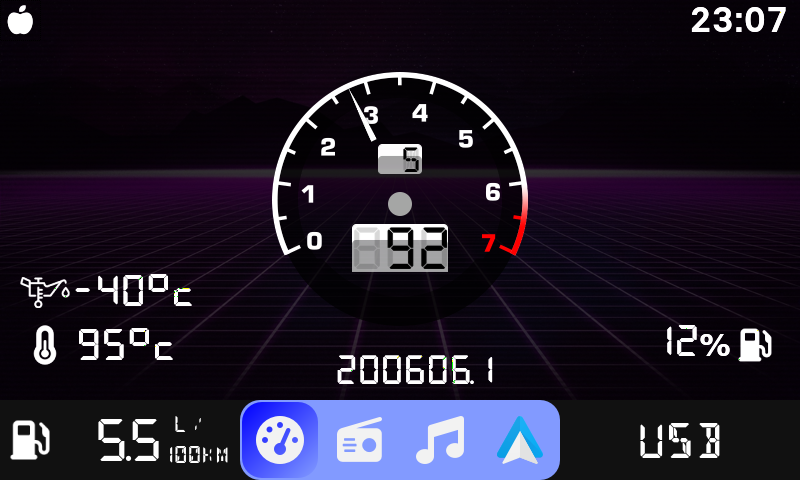
\includegraphics[width=0.75\textwidth]{images/1-rpm.png}
    \caption{Prikaz ekrana tijekom testiranja - Telemetrija automobila}
    \label{fig:car_telemetry}
\end{figure}

Na slici \ref{fig:car_multimedia_external_storage} je prikazan test učitavanja multimedijskog sadržaja sa vanjskog uređaja za pohranu podataka. Kako je sadržaj bez ikakvih problema učitan te reproduciran, zaključuje se kako i taj dio sustava radi kao što je predviđeno.

\begin{figure}[H]
    \centering
    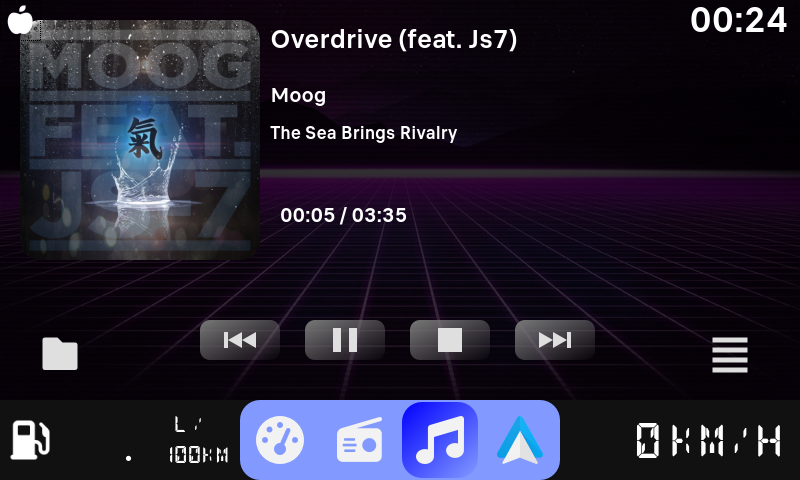
\includegraphics[width=0.75\textwidth]{images/2-musicplayer.png}
    \caption{Prikaz ekrana tijekom testiranja - Multimedija - Uređaj za pohranu podataka}
    \label{fig:car_multimedia_external_storage}
\end{figure}

Na slikama \ref{fig:car_multimedia_radio} i \ref{fig:radio} je prikazan test prikaza aktivne radio stanice (ukoliko je radio upaljen) iz kojih se može vidjeti kako i ta funkcionalnost ima predviđeno ponašanje.

\begin{figure}[H]
    \centering
    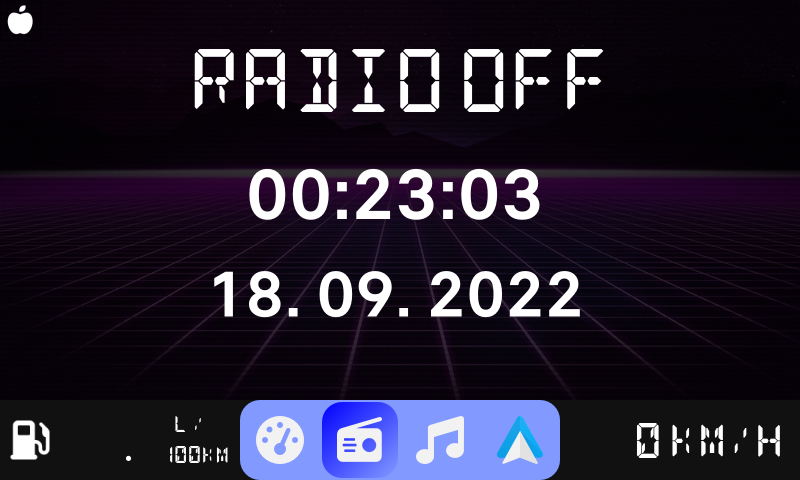
\includegraphics[width=0.75\textwidth]{images/3-radiooff.png}
    \caption{Prikaz ekrana tijekom testiranja - Multimedija - Radio}
    \label{fig:car_multimedia_radio}
\end{figure}

\begin{figure}[H]
    \begin{center}
        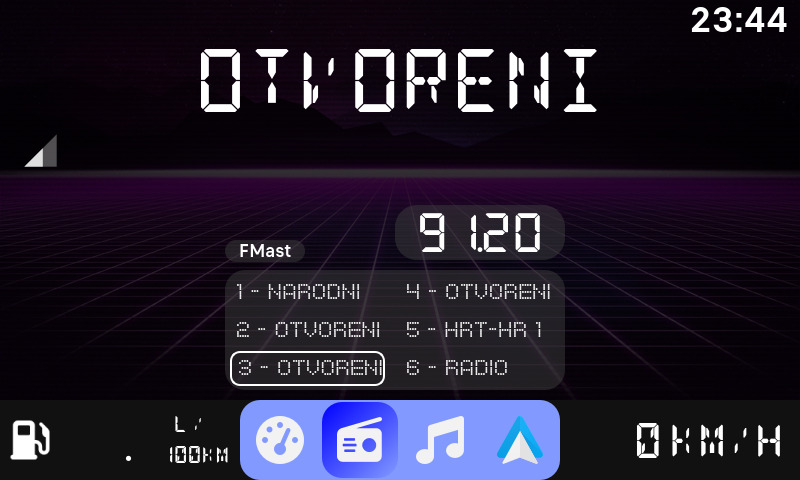
\includegraphics[width=0.75\textwidth]{images/radio.jpeg}
        \caption{Infotainment sustav smješten u autu}
        \label{fig:radio}
    \end{center}
\end{figure}
\newpage

\section{Zaključak}

Realizacija ovog projekta pokazala je da je moguće uspješno integrirati moderan infotainment sustav u starije vozilo koristeći kombinaciju vlastitog hardverskog modula i open-source softverskih alata. Ključni izazovi bili su razumijevanje i implementacija VAN protokola, osiguranje stabilnog napajanja te izrada pouzdanog firmwarea za ESP32 mikroupravljač. Pažljivim dizajnom tiskane pločice, korištenjem provjerenih komponenti i pisanjem modularnog koda, postignuta je robusna i stabilna komunikacija s vozilom. \\

Prednosti rješenja su otvorenost i mogućnost proširenja funkcionalnosti, niska cijena u odnosu na komercijalne alternative te potpuna kontrola nad softverom i hardverom. Sustav se pokazao pouzdanim tijekom testiranja – prikaz telemetrije, statusa vozila i reprodukcija multimedije radili su bez većih odstupanja od tvorničkih pokazivača. Najveći izazovi, poput dekodiranja VAN okvira i implementacije režima štednje energije, uspješno su savladani korištenjem ESP-IDF okvira i pažljivim upravljanjem događajima i zadacima.\\

Ipak, postoje područja za daljnje unaprjeđenje. Potrebno je dodatno optimizirati potrošnju energije u stanju mirovanja kako bi se maksimalno smanjilo pražnjenje akumulatora te doraditi korisničko sučelje na Raspberry Pi računalu radi intuitivnijeg korištenja. Budući razvoj mogao bi uključivati potpunu integraciju s postojećim zaslonom u vozilu, dodavanje bežične povezivosti (Wi-Fi/Bluetooth sinkronizacija s pametnim telefonom) te naprednije funkcije poput OTA (Over-the-Air) nadogradnje softvera. Time bi se sustav dodatno približio funkcionalnosti i fleksibilnosti modernih tvorničkih infotainment rješenja.



% Ne treba biti numerirano
\printbibliography[heading=bibintoc, label=toc:bibliography]

% Ovo treba pun kurac da se builda, zakomentiraj ako smeta
% Nisam siguran jel ovo treba bit numerirano ili ne
\section*{Prilozi i dodaci}
\addcontentsline{toc}{section}{Prilozi i dodaci}

\subsubsection*{P.1 Kompletna shema sklopovlja}


\includepdf[landscape=true,pages={-}]{images/izlaz.pdf}

\subsubsection*{P.2 Kompletan izvorni kod firmware-a na ESP32.}

\begin{code}
    \captionof{listing}{main.c}
    \inputminted[breaklines]{C}{kod/main.c}
\end{code}

\begin{code}
    \captionof{listing}{common.c}
    \inputminted[breaklines]{C}{kod/common.c}
\end{code}

\begin{code}
    \captionof{listing}{init.c}
    \inputminted[breaklines]{C}{kod/init.c}
\end{code}

\begin{code}
    \captionof{listing}{psa\_helper.c}
    \inputminted[breaklines]{C}{kod/psa_helper.c}
\end{code}

\begin{code}
    \captionof{listing}{tss\_task.c}
    \inputminted[breaklines]{C}{kod/tss_task.c}
\end{code}

\begin{code}
    \captionof{listing}{tss463c.c}
    \inputminted[breaklines]{C}{kod/tss463c.c}
\end{code}

\begin{code}
    \captionof{listing}{uart\_task.c}
    \inputminted[breaklines]{C}{kod/uart_task.c}
\end{code}

\begin{code}
    \captionof{listing}{van\_packet\_parser.c}
    \inputminted[breaklines]{C}{kod/van_packet_parser.c}
\end{code}

\begin{code}
    \captionof{listing}{van\_rmt\_rx.c}
    \inputminted[breaklines]{C}{kod/van_rmt_rx.c}
\end{code}

\begin{code}
    \captionof{listing}{van\_rmt\_task.c}
    \inputminted[breaklines]{C}{kod/van_rmt_task.c}
\end{code}

\begin{code}
    \captionof{listing}{include/global\_config.h}
    \inputminted[breaklines]{C}{kod/include/global_config.h}
\end{code}

\begin{code}
    \captionof{listing}{include/global\_init.h}
    \inputminted[breaklines]{C}{kod/include/global_init.h}
\end{code}

\begin{code}
    \captionof{listing}{include/global\_state\_def.h}
    \inputminted[breaklines]{C}{kod/include/global_state_def.h}
\end{code}

\begin{code}
    \captionof{listing}{include/global\_tasks.h}
    \inputminted[breaklines]{C}{kod/include/global_tasks.h}
\end{code}

\begin{code}
    \captionof{listing}{include/mive/common.h}
    \inputminted[breaklines]{C}{kod/include/mive/common.h}
\end{code}

\begin{code}
    \captionof{listing}{include/mive/psa\_helper.h}
    \inputminted[breaklines]{C}{kod/include/mive/psa_helper.h}
\end{code}

\begin{code}
    \captionof{listing}{include/mive/psa\_packet\_defs.h}
    \inputminted[breaklines]{C}{kod/include/mive/psa_packet_defs.h}
\end{code}

\begin{code}
    \captionof{listing}{include/van/tss463\_regs.h}
    \inputminted[breaklines]{C}{kod/include/van/tss463_regs.h}
\end{code}

\begin{code}
    \captionof{listing}{include/van/tss463c.h}
    \inputminted[breaklines]{C}{kod/include/van/tss463c.h}
\end{code}

\begin{code}
    \captionof{listing}{include/van/van\_packet\_iden.h}
    \inputminted[breaklines]{C}{kod/include/van/van_packet_iden.h}
\end{code}

\begin{code}
    \captionof{listing}{include/van/van\_packet\_parser.h}
    \inputminted[breaklines]{C}{kod/include/van/van_packet_parser.h}
\end{code}

\begin{code}
    \captionof{listing}{include/van/van\_rmt\_rx.h}
    \inputminted[breaklines]{C}{kod/include/van/van_rmt_rx.h}
\end{code}

\begin{code}
    \captionof{listing}{include/van\_structs/van\_car\_status\_structs.h}
    \inputminted[breaklines]{C}{kod/include/van_structs/van_car_status_structs.h}
\end{code}

\begin{code}
    \captionof{listing}{include/van\_structs/van\_cd\_changer\_commands\_struct.h}
    \inputminted[breaklines]{C}{kod/include/van_structs/van_cd_changer_commands_struct.h}
\end{code}

\begin{code}
    \captionof{listing}{include/van\_structs/van\_radio\_settings\_struct.h}
    \inputminted[breaklines]{C}{kod/include/van_structs/van_radio_settings_struct.h}
\end{code}

\begin{code}
    \captionof{listing}{include/van\_structs/van\_rpm\_struct.h}
    \inputminted[breaklines]{C}{kod/include/van_structs/van_rpm_struct.h}
\end{code}

\begin{code}
    \captionof{listing}{include/van\_structs/van\_cdc\_emulator\_structs.h}
    \inputminted[breaklines]{C}{kod/include/van_structs/van_cdc_emulator_structs.h}
\end{code}

\begin{code}
    \captionof{listing}{include/van\_structs/van\_dash\_struct.h}
    \inputminted[breaklines]{C}{kod/include/van_structs/van_dash_struct.h}
\end{code}

\begin{code}
    \captionof{listing}{include/van\_structs/van\_radio\_struct.h}
    \inputminted[breaklines]{C}{kod/include/van_structs/van_radio_struct.h}
\end{code}

\begin{code}
    \captionof{listing}{include/van\_structs/van\_trip\_computer\_struct.h}
    \inputminted[breaklines]{C}{kod/include/van_structs/van_trip_computer_struct.h}
\end{code}

\end{document}
